\begin{figure*}[t]
    \centering
    \begin{subfigure}[t]{0.9\linewidth}
        \centering
        
\includegraphics[width=\linewidth]{imgs/bar_general_diff/bar_general_legend_m.crop.pdf}
    \end{subfigure}%
    \vspace*{0.4em}
     \begin{subfigure}[t]{0.32\textwidth}
        \centering
        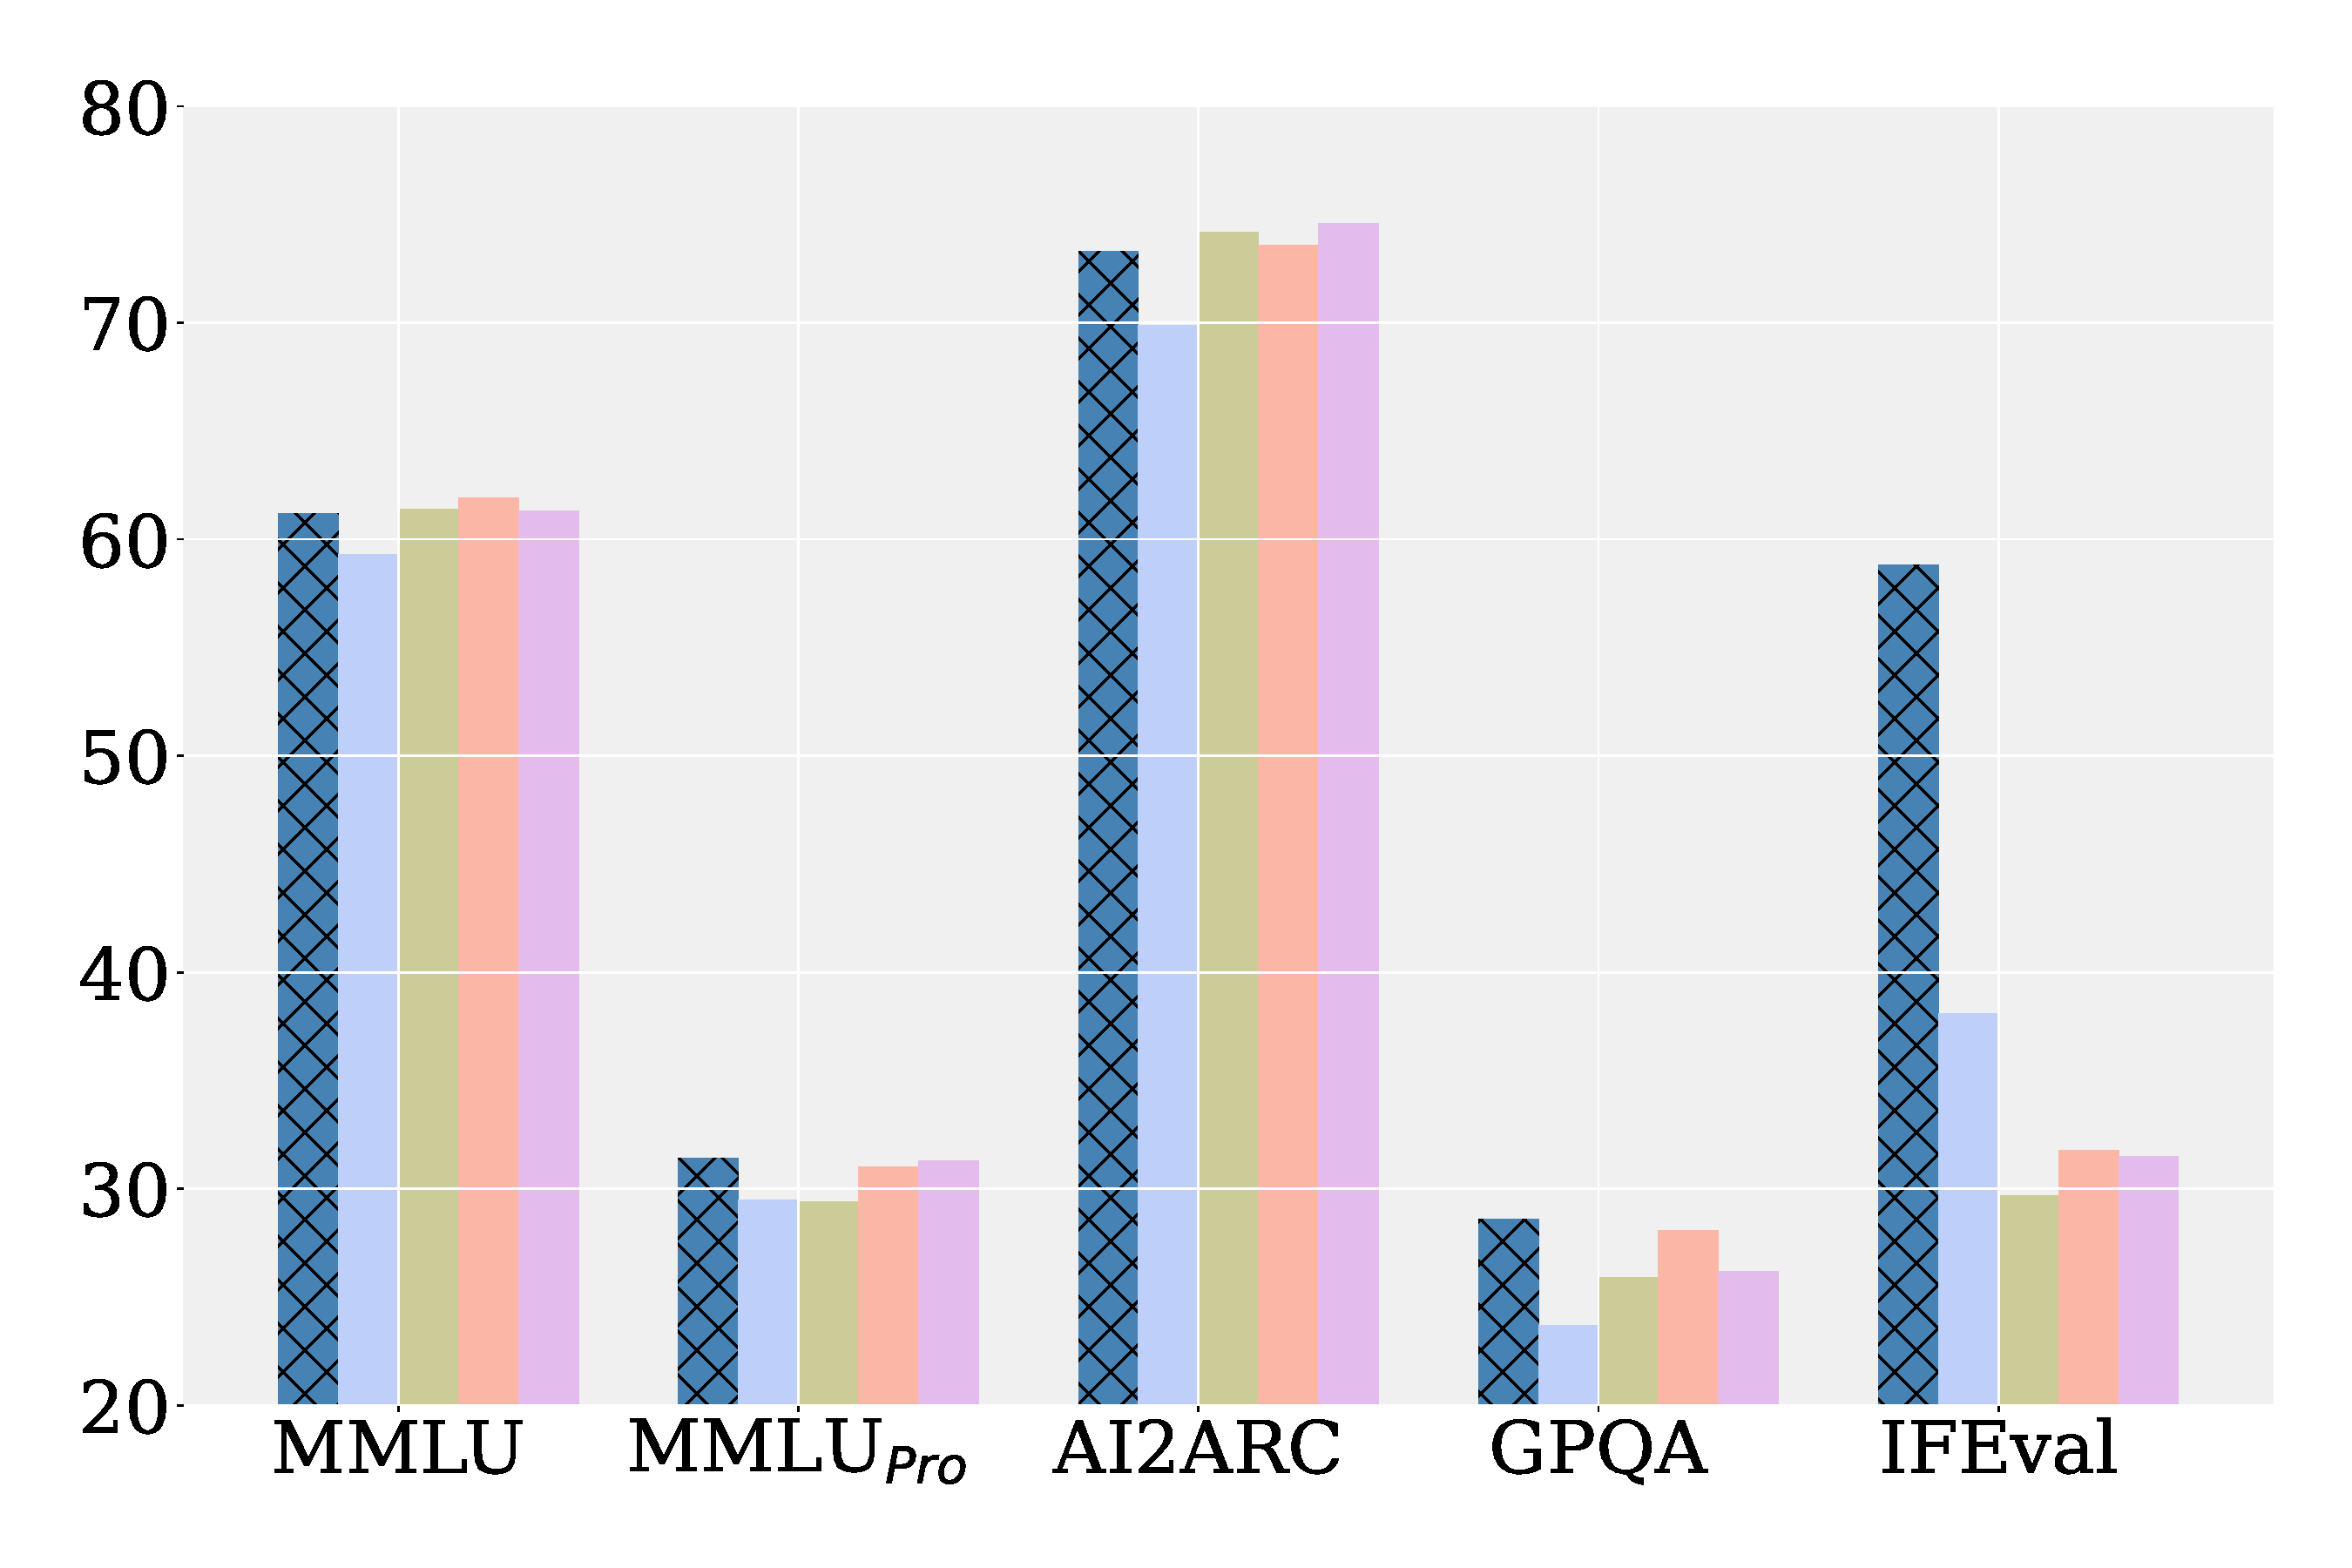
\includegraphics[width=\linewidth]{imgs/bar_general_diff/bar_general_m_modified.pdf}
        \caption{Mistral v0.3 7B Instruct.}
    \end{subfigure}%
    % \hspace{1em}
     \begin{subfigure}[t]{0.32\textwidth}
        \centering
        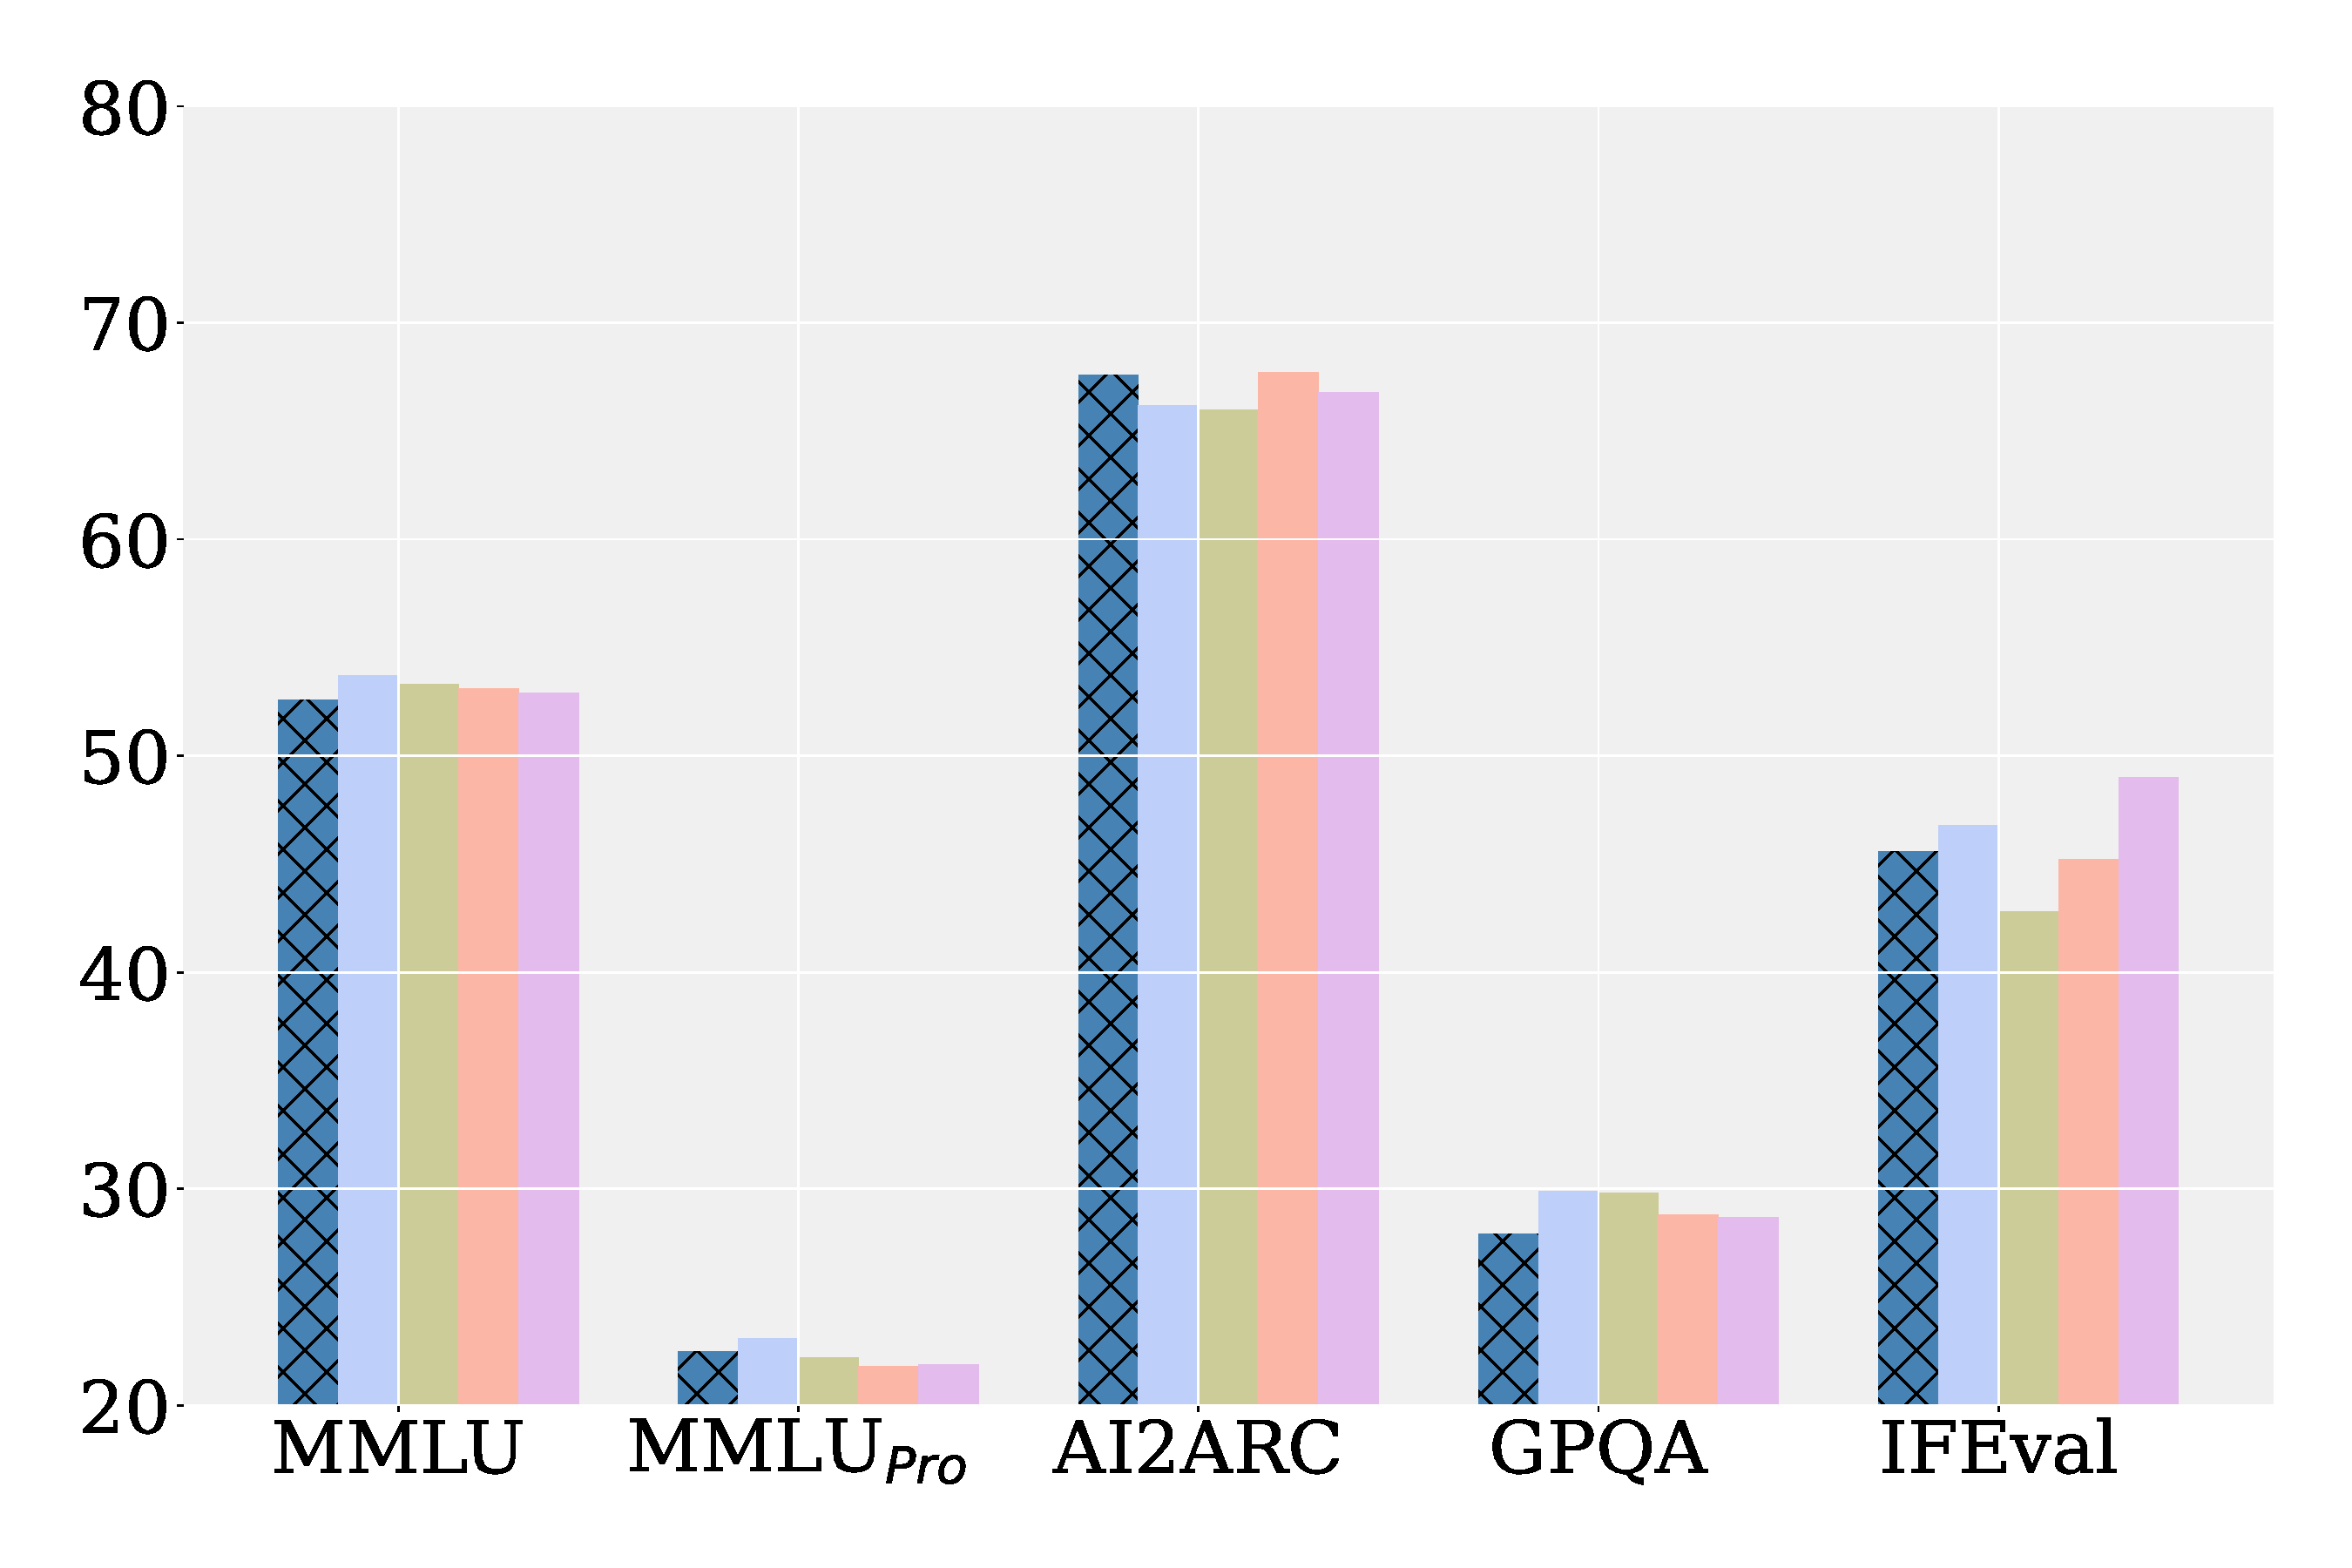
\includegraphics[width=\linewidth]{imgs/bar_general_diff/bar_general_o_modified.pdf}
        \caption{OLMo 7B Instruct.}
    \end{subfigure}%
    % \hspace{1em}
     \begin{subfigure}[t]{0.32\textwidth}
        \centering
        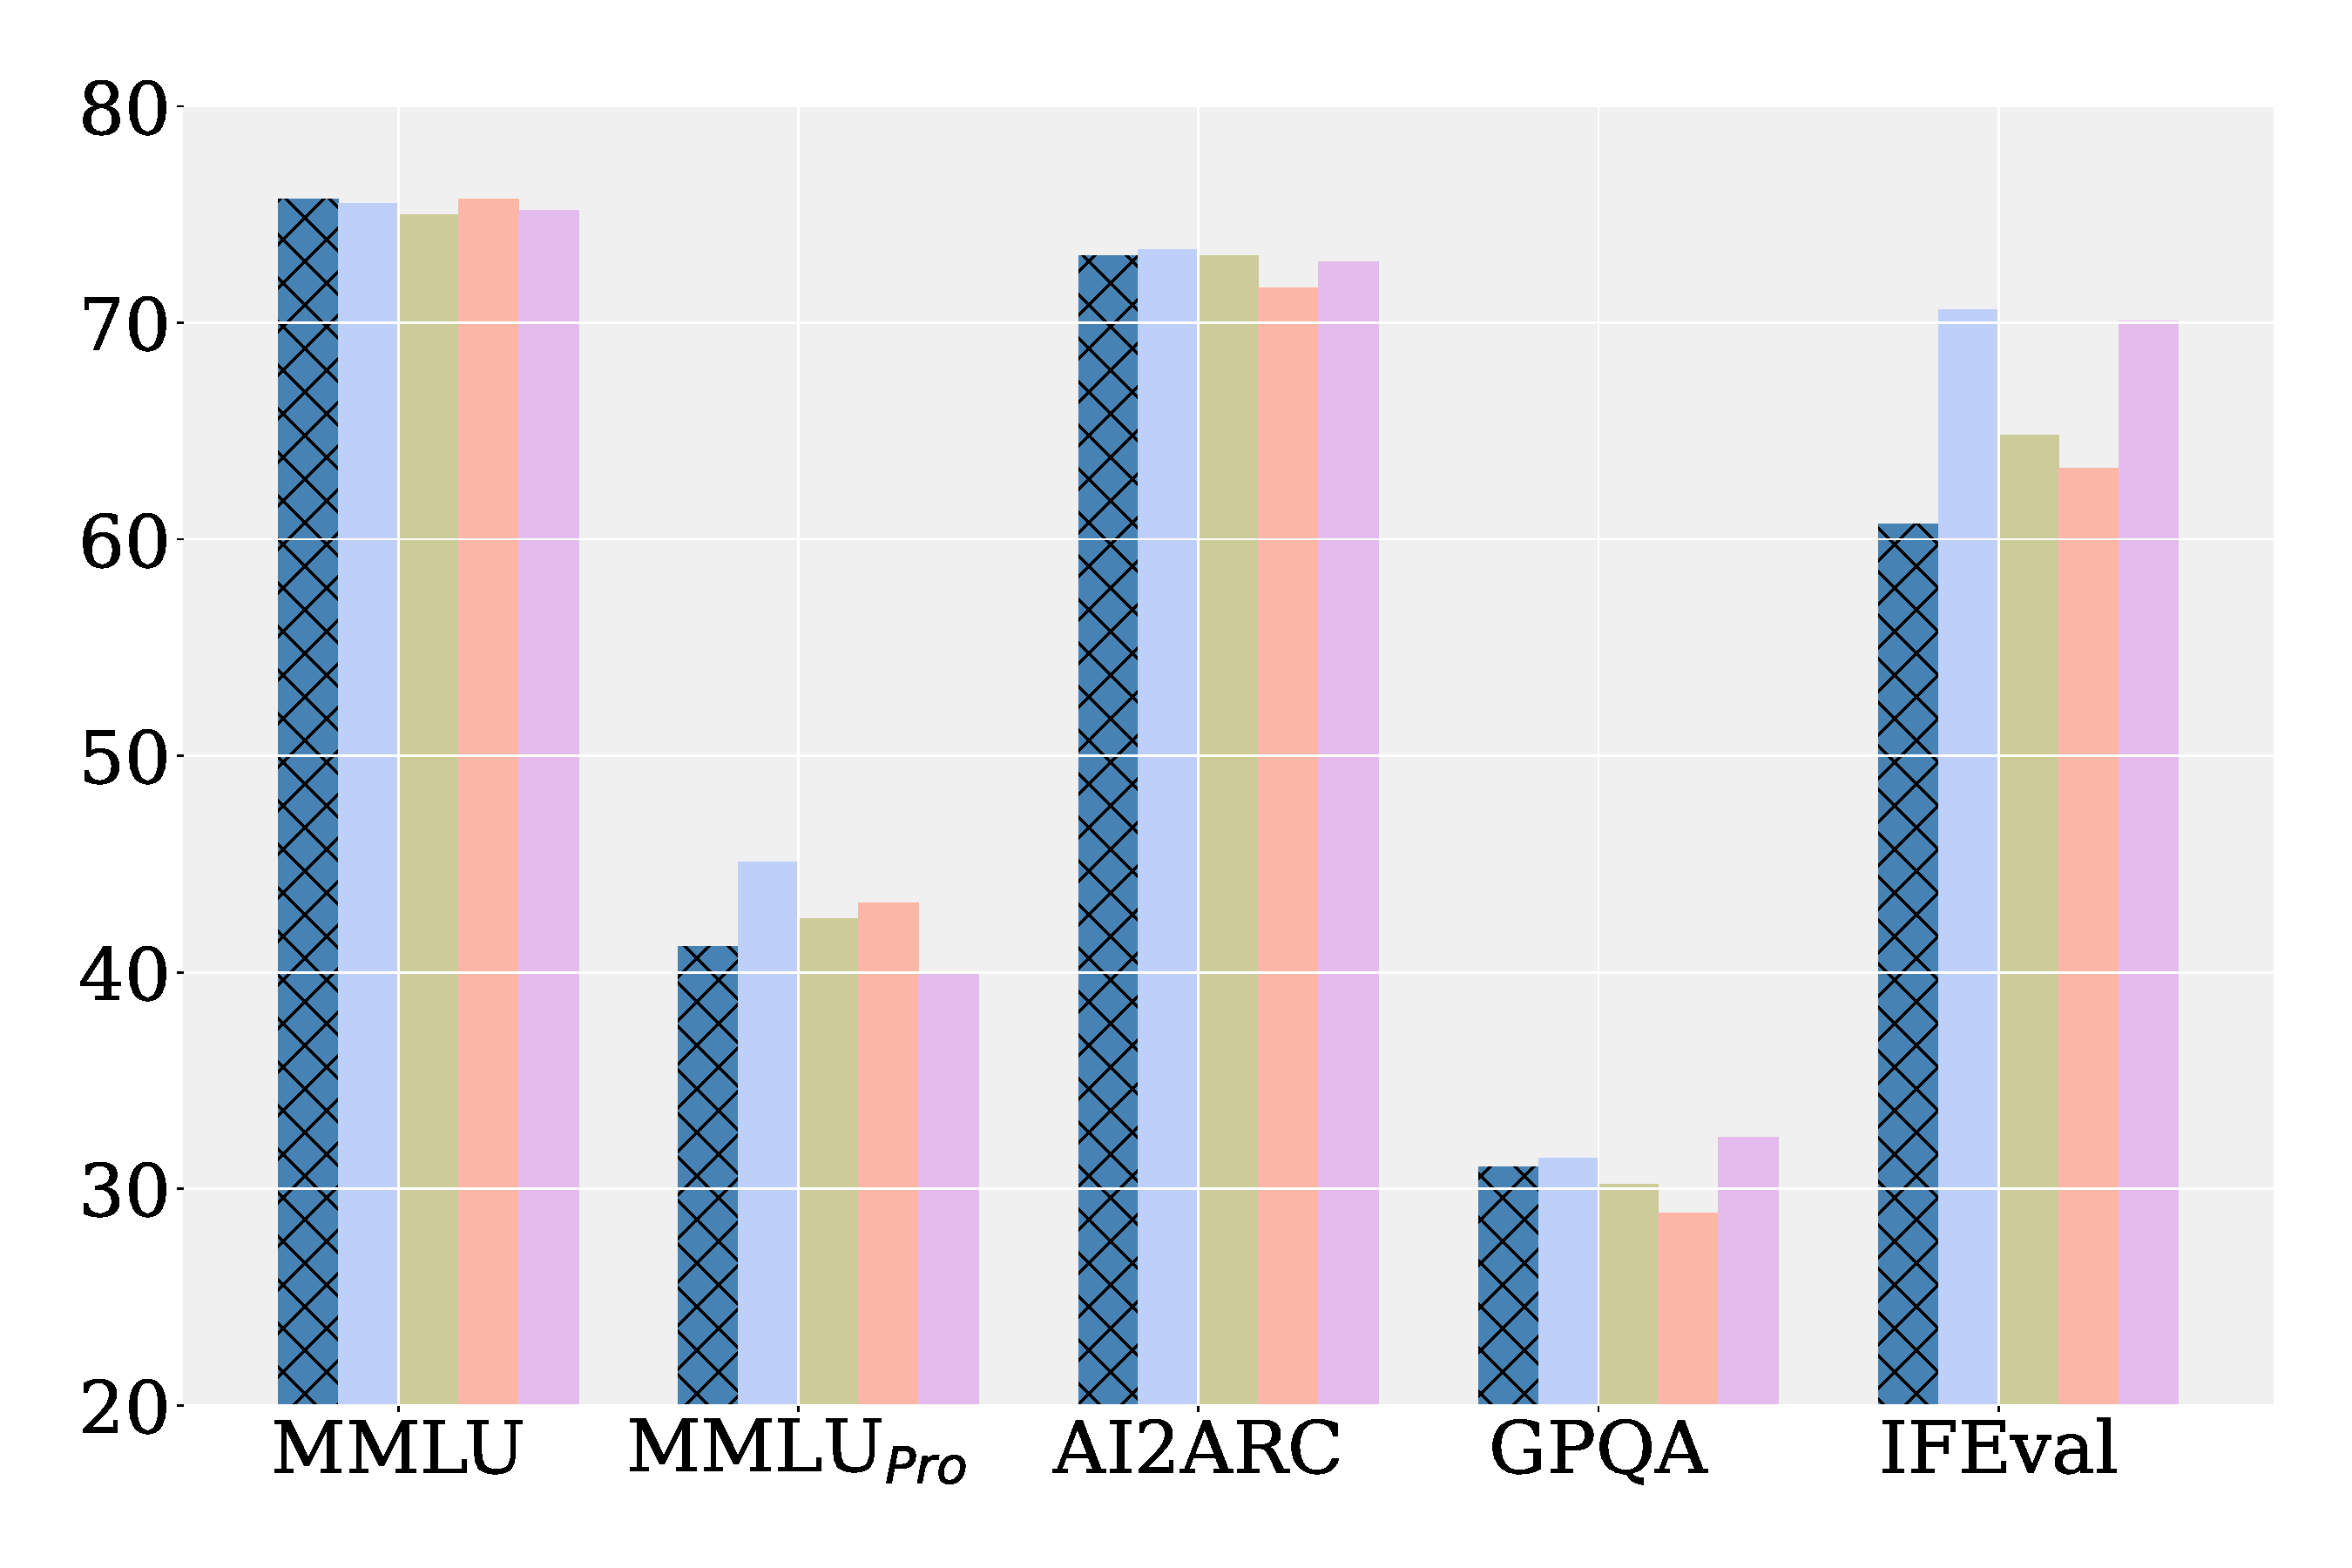
\includegraphics[width=\linewidth]{imgs/bar_general_diff/bar_general_p_modified.pdf}
        \caption{Phi 3 Small Instruct (7B).}
    \end{subfigure}%

    \caption{Performance of fine-tuned models trained on different data (e.g. TableLlama) on general benchmarks. 
    The green and red hatched bars represent performance gains or losses relative to the base model, respectively.
    % We report the difference between the fine-tuned versus the base model for Mistral v0.3 7B Instruct, OLMo 7B Instruct, and Phi 3 Small Instruct (7B).
    % On IFEval, unlike other models, the Mistral model shows a significant performance drop, underscoring the impact of innate model capabilities on preserving general performance after domain-specific fine-tuning.
    % \dnaihao{original capability; select one or two datasets and show; MMLU and IFEval}
    % \dnaihao{use white bar for base model.}
    As indicated by the similar performance bar heights, table instruction tuning does not necessarily compromise the base model's general capabilities.
    \Cref{tab:general} provides the performance in number.
    }
    \label{fig:general-benchmark-performance-difference}
    \vspace{-0.5em}
\end{figure*}